\documentclass{ximera}

 

\usepackage{epsfig}

\graphicspath{
  {./}
  {figures/}
}

\usepackage{morewrites}
\makeatletter
\newcommand\subfile[1]{%
\renewcommand{\input}[1]{}%
\begingroup\skip@preamble\otherinput{#1}\endgroup\par\vspace{\topsep}
\let\input\otherinput}
\makeatother

\newcommand{\includeexercises}{\directlua{dofile("/home/jim/linearAlgebra/laode/exercises.lua")}}

%\newcounter{ccounter}
%\setcounter{ccounter}{1}
%\newcommand{\Chapter}[1]{\setcounter{chapter}{\arabic{ccounter}}\chapter{#1}\addtocounter{ccounter}{1}}

%\newcommand{\section}[1]{\section{#1}\setcounter{thm}{0}\setcounter{equation}{0}}

%\renewcommand{\theequation}{\arabic{chapter}.\arabic{section}.\arabic{equation}}
%\renewcommand{\thefigure}{\arabic{chapter}.\arabic{figure}}
%\renewcommand{\thetable}{\arabic{chapter}.\arabic{table}}

%\newcommand{\Sec}[2]{\section{#1}\markright{\arabic{ccounter}.\arabic{section}.#2}\setcounter{equation}{0}\setcounter{thm}{0}\setcounter{figure}{0}}

\newcommand{\Sec}[2]{\section{#1}}

\setcounter{secnumdepth}{2}
%\setcounter{secnumdepth}{1} 

%\newcounter{THM}
%\renewcommand{\theTHM}{\arabic{chapter}.\arabic{section}}

\newcommand{\trademark}{{R\!\!\!\!\!\bigcirc}}
%\newtheorem{exercise}{}

\newcommand{\dfield}{{\sf dfield9}}
\newcommand{\pplane}{{\sf pplane9}}

\newcommand{\EXER}{\section*{Exercises}}%\vspace*{0.2in}\hrule\small\setcounter{exercise}{0}}
\newcommand{\CEXER}{}%\vspace{0.08in}\begin{center}Computer Exercises\end{center}}
\newcommand{\TEXER}{} %\vspace{0.08in}\begin{center}Hand Exercises\end{center}}
\newcommand{\AEXER}{} %\vspace{0.08in}\begin{center}Hand Exercises\end{center}}

% BADBAD: \newcommand{\Bbb}{\bf}

\newcommand{\R}{\mbox{$\Bbb{R}$}}
\newcommand{\C}{\mbox{$\Bbb{C}$}}
\newcommand{\Z}{\mbox{$\Bbb{Z}$}}
\newcommand{\N}{\mbox{$\Bbb{N}$}}
\newcommand{\D}{\mbox{{\bf D}}}
\usepackage{amssymb}
%\newcommand{\qed}{\hfill\mbox{\raggedright$\square$} \vspace{1ex}}
%\newcommand{\proof}{\noindent {\bf Proof:} \hspace{0.1in}}

\newcommand{\setmin}{\;\mbox{--}\;}
\newcommand{\Matlab}{{M\small{AT\-LAB}} }
\newcommand{\Matlabp}{{M\small{AT\-LAB}}}
\newcommand{\computer}{\Matlab Instructions}
\newcommand{\half}{\mbox{$\frac{1}{2}$}}
\newcommand{\compose}{\raisebox{.15ex}{\mbox{{\scriptsize$\circ$}}}}
\newcommand{\AND}{\quad\mbox{and}\quad}
\newcommand{\vect}[2]{\left(\begin{array}{c} #1_1 \\ \vdots \\
 #1_{#2}\end{array}\right)}
\newcommand{\mattwo}[4]{\left(\begin{array}{rr} #1 & #2\\ #3
&#4\end{array}\right)}
\newcommand{\mattwoc}[4]{\left(\begin{array}{cc} #1 & #2\\ #3
&#4\end{array}\right)}
\newcommand{\vectwo}[2]{\left(\begin{array}{r} #1 \\ #2\end{array}\right)}
\newcommand{\vectwoc}[2]{\left(\begin{array}{c} #1 \\ #2\end{array}\right)}

\newcommand{\ignore}[1]{}


\newcommand{\inv}{^{-1}}
\newcommand{\CC}{{\cal C}}
\newcommand{\CCone}{\CC^1}
\newcommand{\Span}{{\rm span}}
\newcommand{\rank}{{\rm rank}}
\newcommand{\trace}{{\rm tr}}
\newcommand{\RE}{{\rm Re}}
\newcommand{\IM}{{\rm Im}}
\newcommand{\nulls}{{\rm null\;space}}

\newcommand{\dps}{\displaystyle}
\newcommand{\arraystart}{\renewcommand{\arraystretch}{1.8}}
\newcommand{\arrayfinish}{\renewcommand{\arraystretch}{1.2}}
\newcommand{\Start}[1]{\vspace{0.08in}\noindent {\bf Section~\ref{#1}}}
\newcommand{\exer}[1]{\noindent {\bf \ref{#1}}}
\newcommand{\ans}{}
\newcommand{\matthree}[9]{\left(\begin{array}{rrr} #1 & #2 & #3 \\ #4 & #5 & #6
\\ #7 & #8 & #9\end{array}\right)}
\newcommand{\cvectwo}[2]{\left(\begin{array}{c} #1 \\ #2\end{array}\right)}
\newcommand{\cmatthree}[9]{\left(\begin{array}{ccc} #1 & #2 & #3 \\ #4 & #5 &
#6 \\ #7 & #8 & #9\end{array}\right)}
\newcommand{\vecthree}[3]{\left(\begin{array}{r} #1 \\ #2 \\
#3\end{array}\right)}
\newcommand{\cvecthree}[3]{\left(\begin{array}{c} #1 \\ #2 \\
#3\end{array}\right)}
\newcommand{\cmattwo}[4]{\left(\begin{array}{cc} #1 & #2\\ #3
&#4\end{array}\right)}

\newcommand{\Matrix}[1]{\ensuremath{\left(\begin{array}{rrrrrrrrrrrrrrrrrr} #1 \end{array}\right)}}

\newcommand{\Matrixc}[1]{\ensuremath{\left(\begin{array}{cccccccccccc} #1 \end{array}\right)}}



\renewcommand{\labelenumi}{\theenumi)}
\newenvironment{enumeratea}%
{\begingroup
 \renewcommand{\theenumi}{\alph{enumi}}
 \renewcommand{\labelenumi}{(\theenumi)}
 \begin{enumerate}}
 {\end{enumerate}\endgroup}



\newcounter{help}
\renewcommand{\thehelp}{\thesection.\arabic{equation}}

%\newenvironment{equation*}%
%{\renewcommand\endequation{\eqno (\theequation)* $$}%
%   \begin{equation}}%
%   {\end{equation}\renewcommand\endequation{\eqno \@eqnnum
%$$\global\@ignoretrue}}

%\input{psfig.tex}

\author{Martin Golubitsky and Michael Dellnitz}

%\newenvironment{matlabEquation}%
%{\renewcommand\endequation{\eqno (\theequation*) $$}%
%   \begin{equation}}%
%   {\end{equation}\renewcommand\endequation{\eqno \@eqnnum
% $$\global\@ignoretrue}}

\newcommand{\soln}{\textbf{Solution:} }
\newcommand{\exercap}[1]{\centerline{Figure~\ref{#1}}}
\newcommand{\exercaptwo}[1]{\centerline{Figure~\ref{#1}a\hspace{2.1in}
Figure~\ref{#1}b}}
\newcommand{\exercapthree}[1]{\centerline{Figure~\ref{#1}a\hspace{1.2in}
Figure~\ref{#1}b\hspace{1.2in}Figure~\ref{#1}c}}
\newcommand{\para}{\hspace{0.4in}}

\renewenvironment{solution}{\suppress}{\endsuppress}

\ifxake
\newenvironment{matlabEquation}{\begin{equation}}{\end{equation}}
\else
\newenvironment{matlabEquation}%
{\let\oldtheequation\theequation\renewcommand{\theequation}{\oldtheequation*}\begin{equation}}%
  {\end{equation}\let\theequation\oldtheequation}
\fi

\makeatother


\title{Periodic Solutions}

\begin{document}
\begin{abstract}
\end{abstract}
\maketitle

 \label{S:periodic}
\index{periodic solution}

A periodic solution to a system of differential equations 
\begin{equation}  \label{e:genlveceqn}  
\frac{dX}{dt} = F(X)
\end{equation}
is a nonconstant solution such that 
\begin{equation}  \label{e:period}
X(t)=X(t+T)
\end{equation}
for some positive real number $T$.  The smallest positive number $T$
satisfying \eqref{e:period} is called the {\em period\/}\index{period} 
of the periodic solution.  The {\em frequency\/}\index{frequency} is 
the quantity $1/T$.
 
Uniqueness of solutions\index{uniqueness of solutions} to the initial 
value problem has an interesting consequence concerning periodic solutions.
\begin{lemma}  
Let $X(t)$ be a nonconstant solution to the autonomous
system \eqref{e:genlveceqn} such that 
\[
X(T)=X(0).
\]
Then $X(t)$ is a periodic solution with period dividing $T$.
\end{lemma}

\begin{proof}  Let $Y(t)=X(t+T)$.  Then $Y(t)$ is a solution to 
\eqref{e:genlveceqn} since 
\[
\dot{Y}(t) = \dot{X}(t+T)=F(X(t+T))=F(Y(t)).
\]
This solution has initial condition $Y(0)=X(T)=X(0)$.  
Uniqueness of solutions with the same initial condition 
implies that $X(t)=Y(t)$ for all $t$ and that $X(t)=X(t+T)$.
Since $X(t)$ is not an equilibrium, there is a smallest 
positive period for $X$ and that period must divide $T$. \end{proof}

In this section we study two types of planar systems that have periodic 
solutions, centers and phase--amplitude equations, and in both examples 
we prove that the system has periodic solutions.  Typically, however, 
proving that periodic solutions exist is not a simple task; in general 
we rely on numerical solution to verify existence of periodic solutions..




\subsubsection*{Nonhyperbolic Centers}

Nonconstant periodic solutions occur in linear systems only when the
coefficient matrix has purely imaginary eigenvalues, that is,
when the origin is a center.  Therefore, periodic solutions
occur in linear systems only when the equilibrium is
nonhyperbolic, and they occur in infinite families.  For
example, consider the {\em center\/}  \index{center}
\begin{equation}  \label{e:planeper}
\frac{dX}{dt} = \mattwo{0}{-\tau}{\tau}{0}X.
\end{equation}
Solutions of \eqref{e:planeper} are 
\[
X(t) = \mattwo{\cos(\tau t)}{-\sin(\tau t)}{\sin(\tau t)}
{\cos(\tau t)}X_0.
\]
All nonzero solutions of \eqref{e:planeper} are periodic with period
$2\pi/\tau$.  See Figure~\ref{F:planarperiodic}.

\begin{figure*}[htb]
           \centerline{%
           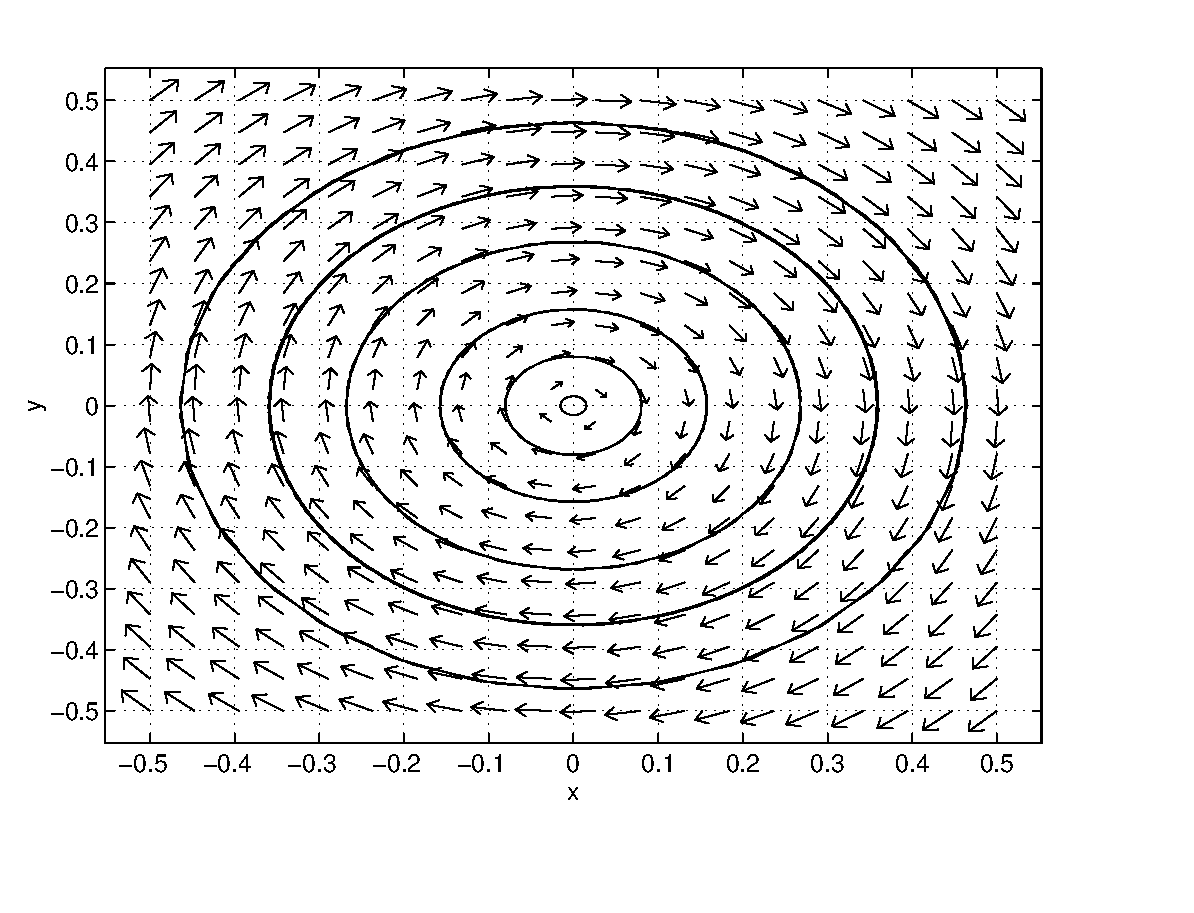
\psfig{file=../figures/periodic.eps,width=3.5in}
           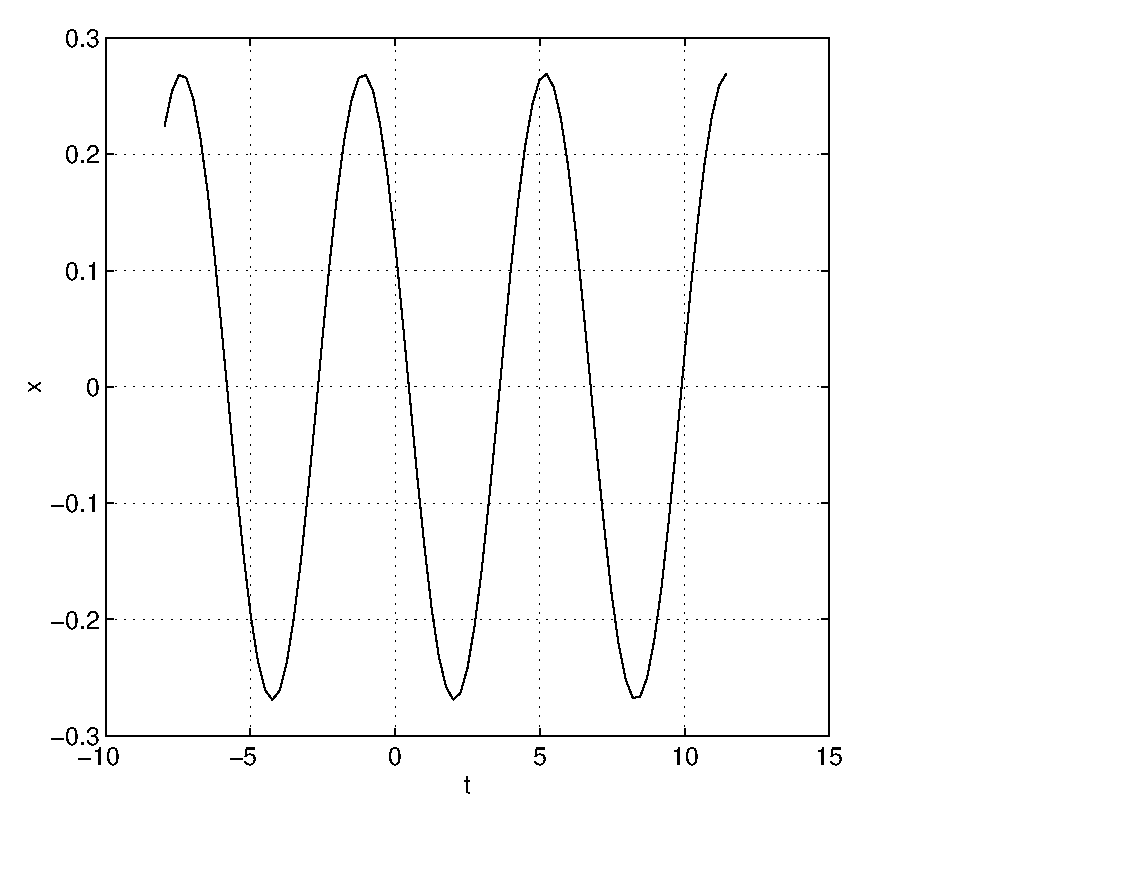
\psfig{file=../figures/period2.eps,width=3.5in}}
           \caption{(Left) Trajectories of \protect\eqref{e:planeper}
	     when $\tau=3$. (Right) A time series of one solution.}
           \label{F:planarperiodic}
\end{figure*}

Centers are examples of nonhyperbolic\index{nonhyperbolic}
equilibria\index{equilibrium!nonhyperbolic}, and higher
order terms will change the 
phase portrait of a center\index{phase!portrait!for a center} --- even
near the origin.  For example, consider the system  \index{hyperbolic}
\begin{matlabEquation}  \label{e:nonlincenter}
\begin{array}{rcl}
\dot{x} & = & -2y -(x^2+y^2)x \\
\dot{y} & = & 2x - (x^2+y^2)y.
\end{array}
\end{matlabEquation}
A trajectory in the phase portrait of \eqref{e:nonlincenter} that
spirals into the origin is shown in Figure~\ref{F:nonlincenter}
(left). Equation \eqref{e:nonlincenter} can be modified to produce
a single periodic solution, as follows:
\begin{matlabEquation}  \label{e:nonlincenter2}
\begin{array}{rcl}
\dot{x} & = & x-2y -(x^2+y^2)x \\
\dot{y} & = & 2x+y - (x^2+y^2)y.
\end{array}
\end{matlabEquation}
See Figure~\ref{F:nonlincenter} (right).  This example shows the necessity 
of assuming hyperbolicity as a hypothesis in Theorem~\ref{T:linearization}.  

\begin{figure*}[htb]
           \centerline{%
           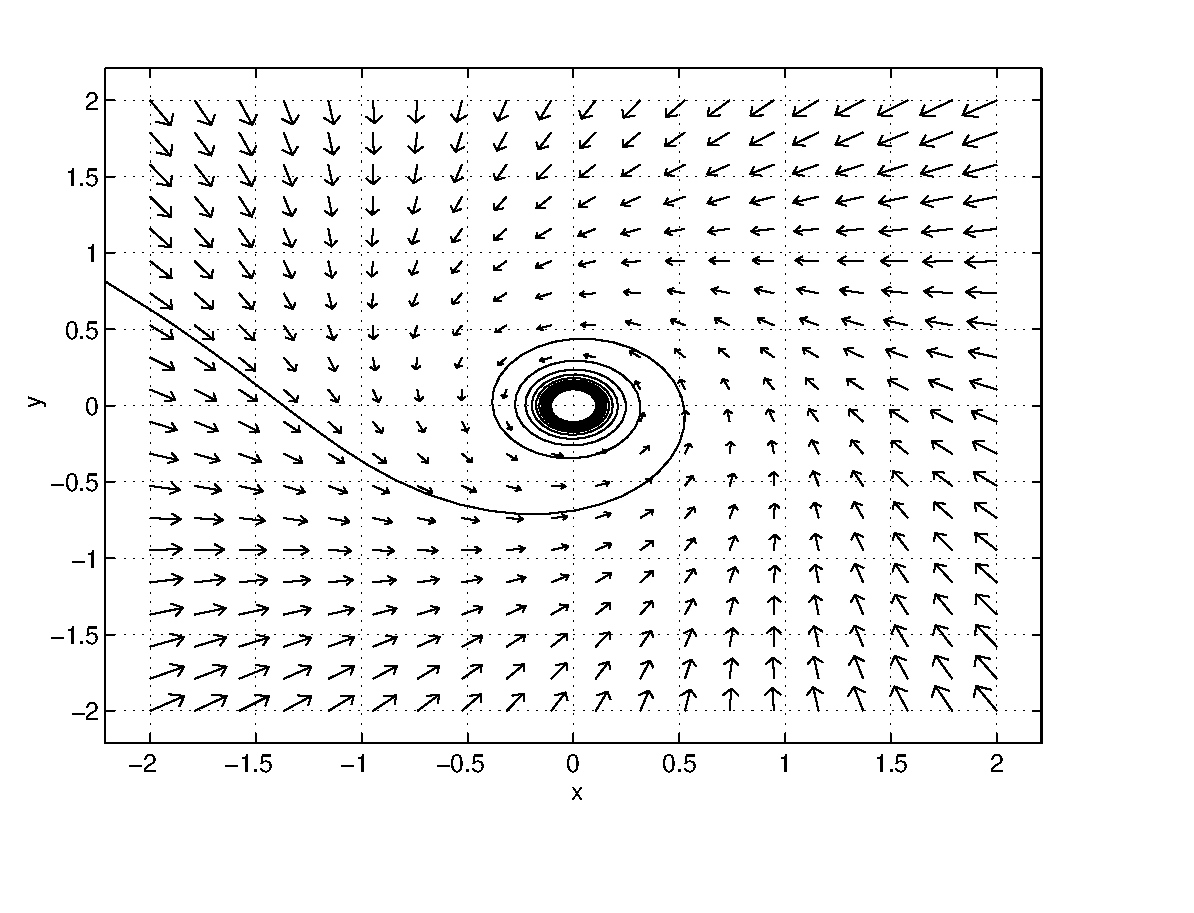
\psfig{file=../figures/period3.eps,width=3.5in}
	   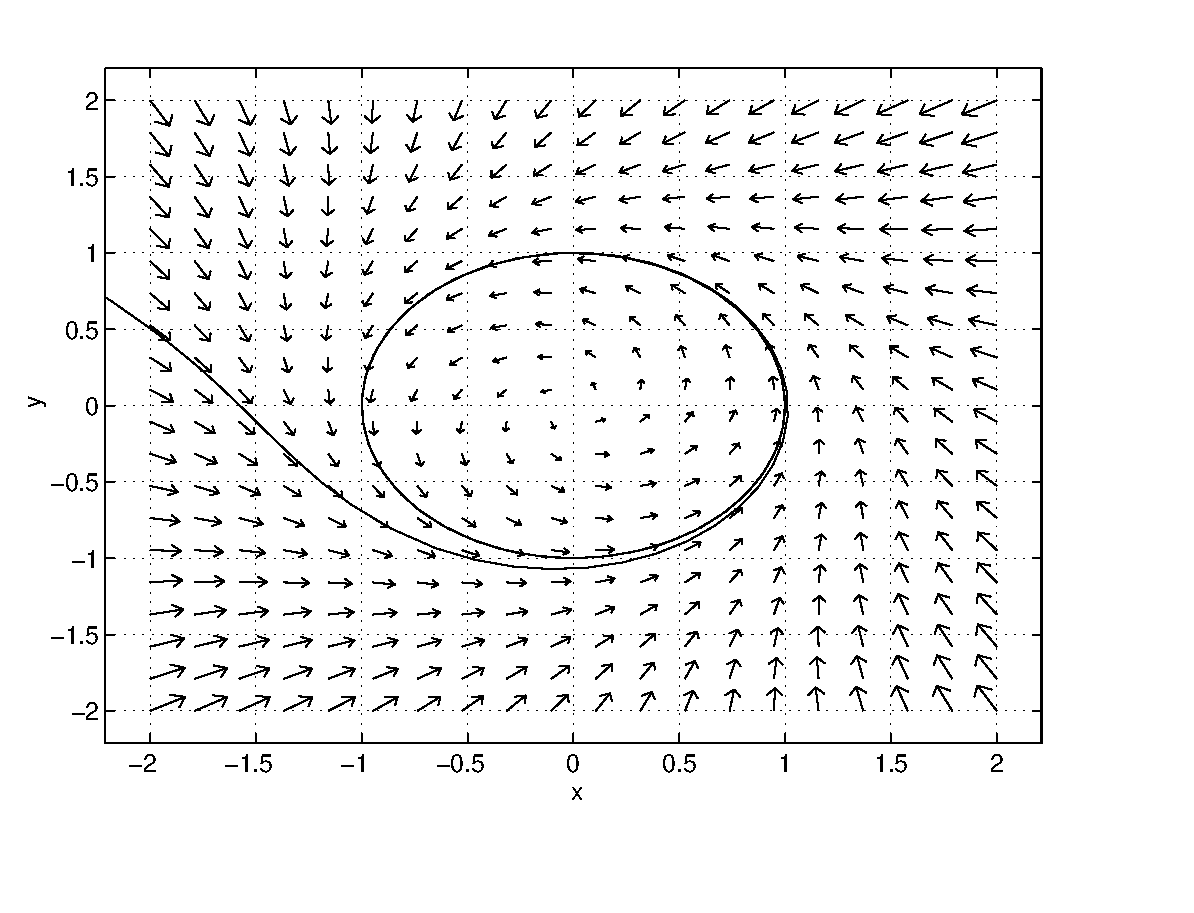
\psfig{file=../figures/period4.eps,width=3.5in}}
           \caption{(Left) A trajectory of \protect\eqref{e:nonlincenter}
that spirals towards the origin. Note the slow convergence due to the fact 
that the origin is not hyperbolic.  (Right) A trajectory of 
\protect\eqref{e:nonlincenter2} that spirals towards a periodic solution.}
           \label{F:nonlincenter}
\end{figure*}

\subsection*{Phase -- Amplitude Equations}
\index{phase-amplitude equations}

We now show why equations \eqref{e:nonlincenter},\eqref{e:nonlincenter2} 
behave as observed in the numerical integration.  We do this using 
polar coordinates\index{polar coordinates} and phase-amplitude equations.  
Recall that rectilinear coordinates $(x,y)$ can be written in terms 
of polar coordinates $(r,\theta)$ as
\begin{eqnarray*}
x & = & r\cos\theta\\
y & = & r\sin\theta.
\end{eqnarray*}
On inverting these equations we find that
\arraystart
\begin{equation} \label{e:polarccord}
\begin{array}{lcl}
r^2 & = & x^2+y^2  \\
\theta & = & \dps\tan\inv\left(\frac{y}{x}\right). 
\end{array}
\end{equation}
\arrayfinish
In applications, $r$ is called the {\em amplitude\/}\index{amplitude} and 
$\theta$ the {\em phase\/}.\index{phase}

Suppose that $(x(t),y(t))$ is the solution to a planar system of
ODEs of the form 
\begin{equation} \label{e:HopfNF}
\begin{array}{rcl}
\dot{x} & = & a(x^2+y^2)x - b(x^2+y^2)y\\
\dot{y} & = & a(x^2+y^2)y + b(x^2+y^2)x,
\end{array}
\end{equation}
where $a$ and $b$ are differentiable functions of $x^2+y^2$.
Note that \eqref{e:nonlincenter} and \eqref{e:nonlincenter2} are special cases 
of \eqref{e:HopfNF}.  In \eqref{e:nonlincenter} $a(r^2)=-r^2$ and $b(r^2)=2$, 
while in \eqref{e:nonlincenter2} $a(r^2)=1-r^2$ and $b(r^2)=2$.

Applying the chain rule\index{chain rule} to \eqref{e:polarccord}, we obtain 
\arraystart
\begin{equation}  \label{e:polarder}
\begin{array}{rcl}
\dot{r} & = & \dps\frac{1}{r}\left(x\dot{x} + y\dot{y}\right)\\ 
\dot{\theta} & = & \dps\frac{1}{r^2}\left(x\dot{y}-y\dot{x}\right).
\end{array}
\end{equation}
\arrayfinish
Substitute the values of $\dot{x}$ and $\dot{y}$ from \eqref{e:HopfNF} into 
\eqref{e:polarder} to obtain the 
{\em amplitude\/} equation\index{amplitude!equation}
\begin{equation} \label{e:amplitude}
\frac{dr}{dt}  =  a(r^2) r
\end{equation}
and the {\em phase\/} equation\index{phase!equation}
\begin{equation} \label{e:phase}
\frac{d\theta}{dt} =  b(r^2).
\end{equation}

\begin{proposition}
Suppose that $r_0$ is a positive zero of the amplitude equation, that is,
$a(r_0^2)=0$.  If $b(r_0^2)\neq 0$, then the circle $r=r_0$ is the
trajectory\index{trajectory} of a periodic solution to \eqref{e:HopfNF}.  

Moreover, if $a'(r^2_0)<0$ then the periodic solution is asymptotically 
stable; if $a'(r^2_0)>0$ then the periodic solution is unstable.
\end{proposition}\index{stability!asymptotic}\index{periodic solution}

\begin{proof}  The function $r(t)$ measures how far the solution $(x(t),y(t))$ to
\eqref{e:HopfNF} is from the origin.  Thus, if $r_0$ is a positive zero of the 
amplitude equation, then the distance of the solution remains constant; that
is, the trajectory of $(x(t),y(t))$ in the plane lies on the circle $r=r_0$
(or $x^2+y^2=r^2$ in Cartesian coordinates).  The solution to the phase 
equation corresponding to this amplitude equilibrium is 
$\theta(t)=b(r_0^2)t+\theta_0$.  Therefore, if $b(r_0^2)\neq 0$, then the 
solution trajectory moves around the circle $r=r_0$ with nonzero constant 
speed.

To verify the statement on asymptotic stability, write the amplitude 
equation as 
\[
\dot{r} = a(r^2)r \equiv f(r).
\]
The point $r_0>0$ is an equilibrium for the amplitude equation if $f(r_0)=0$, 
that is, if $a(r_0^2)=0$.  That equilibrium is asymptotically stable if 
$f'(r_0)<0$.  Using the product rule and the chain rule we see that 
\[
f'(r) = a'(r^2)2r^2 +a(r^2).
\]
Therefore
\[
f'(r_0) = 2r_0^2a'(r_0^2).
\]
It follows that $f'(r_0)<0$ if and only if $a'(r_0^2)<0$.
  
If $a'(r^2_0)<0$, then the equilibrium of the amplitude equation is 
asymptotically stable and nearby trajectories to the planar periodic solution
limit on that periodic solution $r=r_0$ in forward time.  \end{proof} 



\subsubsection*{The Two Examples}

As noted, in both equations \eqref{e:nonlincenter} and \eqref{e:nonlincenter2}
$b(r^2) = 2$.  In the first equation $a(r^2) = -r^2$, while in
the second equation $a(r^2)=1-r^2$.  In both equations, the
phase equation is
\[
\frac{d\theta}{dt} = 2,
\]
that is solved for $\theta = 2t + \theta_0$ for some initial
$\theta_0$.  Thus all solutions spin around the origin
counterclockwise at a constant speed.  In \eqref{e:nonlincenter}
the amplitude equation is
\[
\frac{dr}{dt} = -r^3,
\]
and all solutions approach $r=0$ in forward time.  Thus, the 
phase-amplitude equations together imply that all solutions 
to \eqref{e:nonlincenter} spiral into the origin, even though the 
origin in the linearized equations is a center. 

In \eqref{e:nonlincenter2} the amplitude equation is 
\[
\frac{dr}{dt} = r-r^3.
\]
In this equation all solutions with positive initial $r$ tend towards 
$r=1$, the unit circle in the $xy$-plane.  This is seen using the one
dimensional phase line: note that there is only one positive equilibrium at 
$r=1$ and that solutions diverge from $0$ and $\infty$.  Thus, the 
phase-amplitude equations\index{phase-amplitude equations} show that 
all solutions (except the origin) spiral in forward time counterclockwise 
into the unit circle (that is a periodic solution).

\subsection*{Limit Cycles}
\index{limit cycle}

In general, for nonlinear systems without special structure, 
we do not expect periodic solutions to come in continuous families.
We do expect periodic solutions to be isolated --- as in 
Figure~\ref{F:globalb} (left).  

We call a periodic solution $x(t)$ a {\em limit cycle\/} if all 
nearby trajectories converge to $x(t)$ in forward time or all nearby
solutions converge to $x(t)$ in backward time.  Note that in phase 
space a limit cycle is always isolated; in particular, a limit cycle 
cannot be included in a continuous family of periodic solutions as 
happens in \eqref{e:planeper}.

\begin{theorem} \label{T:PB}
Suppose that the right hand side of a planar system of differential 
equations is defined and smooth everywhere inside a periodic solution.  
Then there is an equilibrium inside the periodic solution.
\end{theorem} 
\index{periodic solution!equilibrium inside}

This theorem is a consequence of the celebrated Poincar\'e-Bendixson theorem
\index{Poincar\'e-Bendixson theorem} and simplifies the search for limit 
cycles in the plane; limit cycles must surround at least one equilibrium.  
Again, the most important information for determining the dynamics of a given 
planar differential equation is the number and type of equilibria.  Once the 
equilibria are known, more complicated features, such as periodic 
solutions and stable and unstable orbits at saddles, can be found by 
exploration.

\EXER

\includeexercises

\end{document}
